% math.tex — \input'd from thesis/experiments.tex
%
% Lagrangian products of rotated 2D polygons: systematic search for
% Viterbo counterexamples in the space of Lagrangian products.
%
% Sources:
%   - Generated data: experiments/lagrangian-products/lagrangian-products-5x5.jsonl
%     and experiments/lagrangian-products/lagrangian-products-<n>x<m>-6deg.jsonl
%   - HK-O 2024 counterexample: Haim-Kislev & Ostrover, Annals 2024
%   - Symmetry analysis: agent-written, Jörn-confirmed direction
%
% Structure:
%   - Mathematical setup (Lagrangian products, rotation parameter)
%   - Symmetry lemma (fundamental domain)
%   - Pentagon rotation curve (Family 1)
%   - Regular polygon grid (Family 2)
%   - Random Lagrangian products (Family 3)
%   - Findings

\subsection{Lagrangian Products of Rotated Polygons}
\label{sec:lagrangian-products}

The only known 4D counterexample to Viterbo's conjecture is a Lagrangian
product of two pentagons \cite{HaimKislevOstrover2024}.
Our sample of random 4-polytopes never exceeded~$\mathrm{sys} > 1$. 
We now probe the conjecture by searching systematically in the space of Lagrangian products, where counterexamples are known to exist.

\subsubsection*{Mathematical setup}

Recall (Definition~\ref{def:lagrangian-product}) that the Lagrangian product
of convex polygons~$P \subset \mathbb{R}^2_q$ and~$Q \subset \mathbb{R}^2_p$
is $P \times_L Q = \{(q,p) : q \in P,\, p \in Q\} \subset \mathbb{R}^4$.

The 4-volume satisfies~$\operatorname{vol}_4(P \times_L Q)
= \operatorname{area}(P) \cdot \operatorname{area}(Q)$ (Fubini's theorem on
complementary subspaces).

\paragraph{Rotation parameter.}
Fix a polygon~$P$ in $q$-space. For an angle~$\theta$, let~$R(\theta)$ denote
the standard rotation in~$\mathbb{R}^2$ and
define~$Q_\theta = R(\theta)\,Q$. We study the one-parameter family
\[
  K_\theta \;=\; P \times_L Q_\theta.
\]
Since rotating both factors by the same angle~$\varphi$ is a symplectic
transformation~$\operatorname{diag}(R(\varphi), R(\varphi)) \in \mathrm{Sp}(4)$,
only the \emph{relative} rotation between the factors affects~$\mathrm{sys}$.

\begin{lemma}[Fundamental domain for rotation sweeps]
\label{lem:rotation-fundamental-domain}
Let~$P$ be a regular $n$-gon and~$Q$ a regular $m$-gon, both centered at the
origin. Then~$\mathrm{sys}(P \times_L Q_\theta)$ depends on~$\theta$ only
through its equivalence class in~$[0, \pi/\operatorname{lcm}(n,m)]$.
\end{lemma}

\begin{proof}
\emph{Periodicity.}
The block-diagonal matrix~$M_\varphi = \operatorname{diag}(R(\varphi),
R(\varphi))$ is symplectic (direct verification: $M_\varphi^T J_0 M_\varphi
= J_0$). Applying~$M_{2\pi/n}$ to~$P \times_L Q_\theta$
maps~$P$ to itself ($n$-fold rotational symmetry)
and replaces~$Q_\theta$ with~$Q_{\theta + 2\pi/n}$. Similarly, the $m$-fold symmetry of~$Q$
gives $Q_\theta = Q_{\theta + 2\pi/m}$. The combined periodicity
is~$2\pi/\operatorname{lcm}(n,m)$.

\emph{Mirror symmetry.}
The matrix~$M = \operatorname{diag}(-1, 1, -1, 1)$ is symplectic
(verification:~$M^T J_0 M = J_0$). It acts on~$\mathbb{R}^2_q$ as reflection
across the~$q_2$-axis and on~$\mathbb{R}^2_p$ as reflection across
the~$p_2$-axis. For our angle convention (normals starting at~$\pi/2$), both
regular polygons are invariant under these reflections, and~$M$
maps~$Q_\theta$ to~$Q_{-\theta}$.

Together: $\mathrm{sys}(\theta)$ has period~$2\pi/\operatorname{lcm}(n,m)$ and
satisfies~$\mathrm{sys}(\theta) = \mathrm{sys}(-\theta)$, so the fundamental
domain is~$[0, \pi/\operatorname{lcm}(n,m)]$.
\end{proof}

% Factor swap: N = -J_0 is symplectic, maps P x_L Q to Q x_L (-P).
% For centrally symmetric polygons, swapping factors preserves sys.
% For odd polygons, -P = R(π)P so the swap also rotates one factor by 180°.
% (Jörn verified 2025-02-14.)

\subsubsection*{Family 1: Pentagon rotation curve}

We sweep the fundamental domain~$\theta \in [0^\circ, 36^\circ]$ at~$1^\circ$ resolution (37 points)
for the family~$\mathrm{Pentagon} \times_L R(\theta)\,\mathrm{Pentagon}$,
where each pentagon is regular with circumradius~1.
We compute~$c_{\mathrm{EHZ}}$ using the billiard algorithm, which is the production-fast method for Lagrangian
products.

Figure~\ref{fig:pentagon-sweep} shows the resulting curve.

The maximum~$\mathrm{sys} \approx 1.0472$ occurs at~$\theta \equiv 18^\circ
\pmod{36^\circ}$ (equivalently $\theta = 90^\circ$, the HK-O angle).
The minimum~$\mathrm{sys} \approx 0.9472$ occurs
at~$\theta \equiv 0^\circ \pmod{36^\circ}$ (aligned or maximally rotated
pentagons). The violation region $\mathrm{sys} > 1$ spans
approximately~$\theta \in (13.5^\circ, 22.5^\circ)$ within each fundamental
domain---about~$25\%$ of the period.

\begin{figure}[h]
\centering
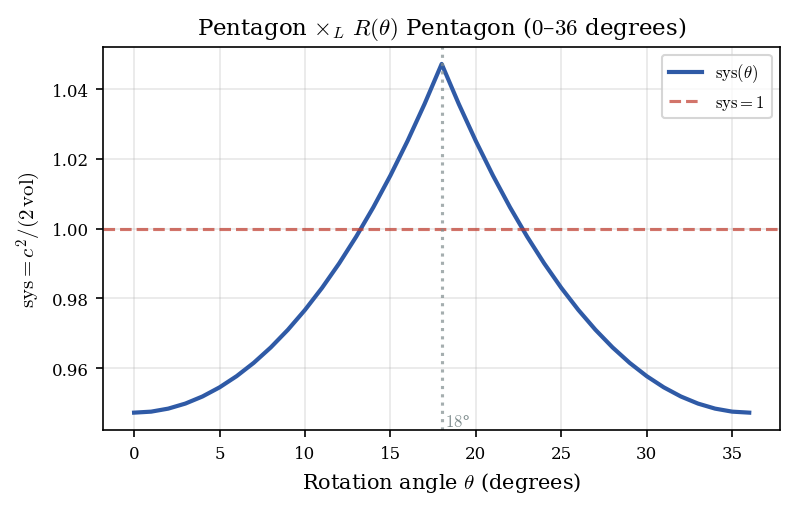
\includegraphics[width=0.9\textwidth]{../experiments/lagrangian-products/lagrangian_products_5x5.png}
\caption{Systolic ratio of $\mathrm{Pentagon} \times_L R(\theta)\,
  \mathrm{Pentagon}$ as a function of rotation angle~$\theta$ on the
  fundamental domain $[0^\circ, 36^\circ]$. The red dashed line marks
  $\mathrm{sys} = 1$ (Viterbo threshold).}
\label{fig:pentagon-sweep}
\end{figure}

\subsubsection*{Family 1b: Heptagon rotation curve}

We repeat the fine sweep for the regular heptagon ($n = 7$). The fundamental
domain is $[0^\circ, 180^\circ/7 \approx 25.71^\circ]$
(Lemma~\ref{lem:rotation-fundamental-domain}), sampled at~$26$ equal steps
($\approx 0.99^\circ$ resolution). Data: \texttt{lagrangian-products-7x7.jsonl}
(27~rows).

The curve peaks at $\theta \approx 12.9^\circ$ with $\mathrm{sys} \approx 0.917$,
well below~$1$. No counterexample.

\begin{figure}[h]
\centering
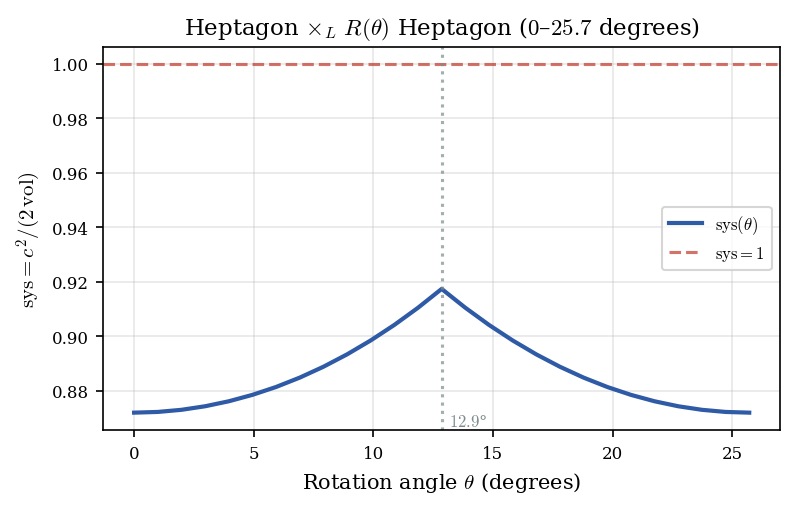
\includegraphics[width=0.9\textwidth]{../experiments/lagrangian-products/lagrangian_products_7x7.png}
\caption{Systolic ratio of $\mathrm{Heptagon} \times_L R(\theta)\,
  \mathrm{Heptagon}$ as a function of rotation angle~$\theta$ on the
  fundamental domain $[0^\circ, 25.7^\circ]$. The red dashed line marks
  $\mathrm{sys} = 1$ (Viterbo threshold).}
\label{fig:heptagon-sweep}
\end{figure}

\subsubsection*{Family 2: Regular polygon pairs}

We sweep the rotation angle for the regular pairs
$(3,3)$, $(3,4)$, $(3,5)$, $(3,6)$, $(4,4)$, $(4,5)$, $(4,6)$, $(5,5)$,
$(5,6)$, and $(6,6)$. For each pair, we sample the fundamental domain
$[0^\circ, 180^\circ/\operatorname{lcm}(n,m)]$ at~$6^\circ$ steps.
Each pair is stored in its own JSONL file
\texttt{lagrangian-products-\emph{n}x\emph{m}-6deg.jsonl} and computed using
the billiard algorithm only.

Figure~\ref{fig:polygon-pairs} shows the resulting curves.

\begin{figure}[h]
\centering
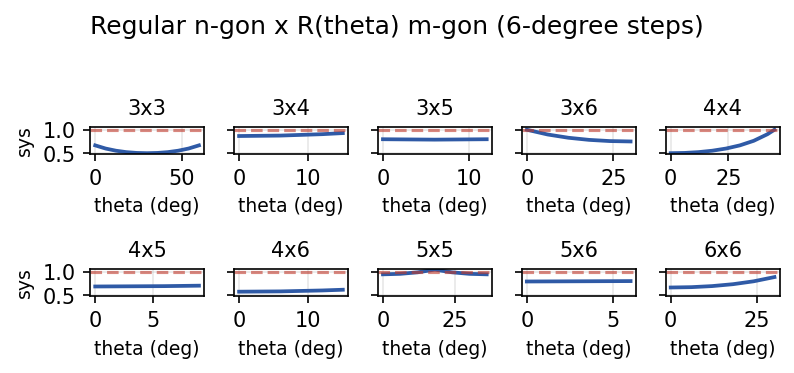
\includegraphics[width=0.95\textwidth]{../experiments/lagrangian-products/lagrangian_products_polygon_pairs.png}
\caption{Systolic ratio curves for regular $n$-gon $\times_L$ $R(\theta)$
  $m$-gon, for the 10 selected pairs. The dashed line marks $\mathrm{sys} = 1$.}
\label{fig:polygon-pairs}
\end{figure}
%
% Legacy experiment sections (commented out for now):
% - Family 3: Random Lagrangian products
% - Aggregate findings list
%
